\subsection{Tracing the September 2020 7(a) reversal}
The twelve portfolios share an issue date and have different ages. Their forecasts draw on twenty disbursement vintages, 2014Q1--2018Q4. We hold the twelve September 2025 outcomes fixed throughout. We separate revisions to the target portfolio's eligible count, its count of charge-offs dated by September 2020, and the donors' dated charge-off histories. We substitute each input from the later edition in all six possible orders and average its marginal change in the MAE gap. The contributions are $+0.006$, $+0.332$ and $+0.062$ pp, respectively. Changing the target event counts alone moves the gap from $-0.185$ to $+0.156$ pp. Thus most of the shift enters through charge-offs recorded for the portfolios being forecast.

The public releases share no agency loan identifier. Our first pass links records uniquely on borrower name, ZIP, approval date and gross approval. It identifies 345 records with a visible charge-off date in 2020 and a blank date in 2025 across the twenty input vintages. Substituting just these changes makes the gap positive ($+0.051$ pp). Averaging the marginal changes over all orders of record-type substitution, the contributions under this literal-key rule from these dates and the unmatched residual are $+0.196$ and $+0.198$ pp.

Because the literal key links only 39.4\% of the eligible 2020 records, we added a second pass after inspecting that residual. It accepts a unique normalized-name match or agreement of two unique keys using the borrower's street and the disbursement date, respectively. The street and disbursement keys also require the same bank. All alternatives require the same approval date, amount and normalized ZIP, and conflicting candidates remain unlinked. This links 229,848 of 261,820 eligible 2020 records (87.8\%). Among linked records, 602 visible dates become blank, including 400 originally dated in 2018--19. Six blank dates become visible and seven visible dates move past the cutoff. The visible-to-blank changes account for $+0.325$ pp of the total. Making only these changes gives a gap of $+0.148$ pp, while making all other changes gives $-0.101$ pp. Unlinked records contribute $+0.063$ pp. All remaining field changes together contribute $+0.012$ pp. The supplement gives both linkage specifications, event quarters and the full ledger.

Both ledgers recover the change in each eligible count and every observable quarterly charge-off cell used in the forecasts. A date that becomes blank removes an event from the recorded endpoint. These files do not establish why the date changed, whether the borrower recovered or whether the agency reversed a loss.

\paragraph{Does the reversal depend on one or two vintages?}
Deleting each target in turn preserves the sign reversal in all twelve comparisons. It also survives all 66 two-target omissions. Across those omissions, archived gaps range from $-0.281$ to $-0.057$ pp and replay gaps from $+0.080$ to $+0.291$ pp. The two largest individual shifts, for 2017Q3 and 2017Q4, account for 42\% of the total. Figure~\ref{fig:revision} shows that four of the twelve target-specific gaps switch strictly from negative to positive, all in 2017. The portfolio-average reversal survives removing the influential quarters even though it is unevenly distributed.

\begin{figure}[htbp]
\centering
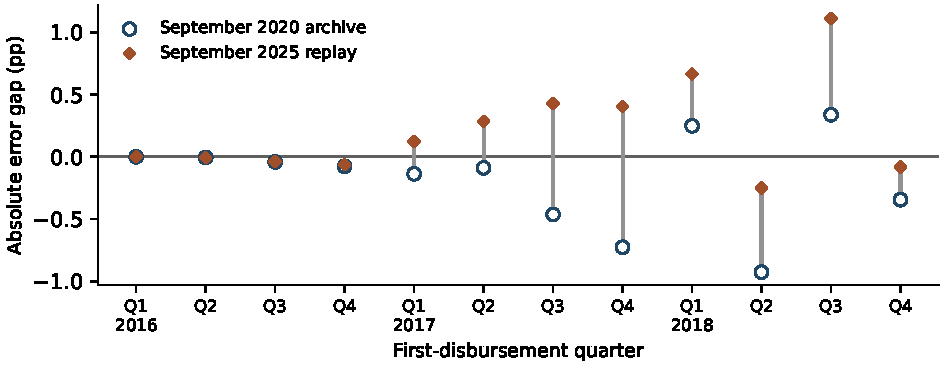
\includegraphics[width=.91\linewidth]{revision_gaps.pdf}
\caption{Recent minus mature absolute error for each September 2020 7(a) target. Each pair uses the same outcome. Points below zero favor recent development factors. For the oldest target only age twenty remains and both rules use the same donors.}
\label{fig:revision}
\end{figure}

Target deletion holds each remaining forecast fixed. A different question is whether revisions to a single input vintage, reused by several forecasts, could explain the pooled sign change. Restoring any one of the twenty input vintages to its archived values preserves the reversal, as does restoring any pair (190 of 190). The smallest replay gap is $+0.063$ pp after restoring 2017Q3 and 2017Q4 together. Conversely, starting from the archive, updating only one input vintage or only two never reverses the ranking. The closest pair is again 2017Q3 and 2017Q4 ($-0.035$ pp). These are exhaustive perturbations of one dated portfolio comparison. The cases share data and do not supply independent economic episodes.
